\documentclass[pdftex,12pt,a4paper]{article}

\usepackage{wrapfig, amssymb, amsmath, graphicx, subfigure, tikz, float, minted}
\usepackage[dutch]{babel}
\usepackage[top=0.5in, bottom=0.5in, left=1in, right=1in]{geometry}
\pagenumbering{arabic}
\newcommand{\HRule}{\rule{\linewidth}{0.5mm}}
\begin{document}
\begin{titlepage}

% Upper part of the page
\begin{flushleft}

\includegraphics[trim=23mm 0mm 0mm 0mm, width=1\textwidth]{./logo.jpg}\\[1cm] \end{flushleft}
\begin{center}
	\textsc{\Large Kansrekening en Statistiek}\\[0.5cm]

    % Title
    \HRule \\[0.4cm] { \huge \bfseries LAB-2}\\[0.4cm]

    \HRule \\[1.5cm]

    % Author and supervisor
\begin{minipage}{0.4\textwidth}
\begin{flushleft} \large \emph{Authors:}\\
Abe \textsc{Wiersma}\\
Stein \textsc{van Zwoll}\\
\end{flushleft}
\end{minipage}
\begin{minipage}{0.4\textwidth} \begin{flushright} \large \end{flushright}\end{minipage}

    \vfill

    % Bottom of the page 
    {\large \today}

\end{center}
\end{titlepage}
\pagebreak

\section*{19 Exercise: Transforming multivariate rv's}
	$$X=(X_1,X_2)^T$$
    $$\mu_{\vec{X}} =
    	\begin{pmatrix}
    		1\\
    		-1
    	\end{pmatrix}
    \textit{ and }  
    \Sigma_{\vec{X}} =
    	\begin{pmatrix}
    		1 & 0\\
    		0 & 4
    	\end{pmatrix}$$
    \\
    $$E(\vec{Z}) = E
    	\begin{pmatrix}
    		Z_1\\
    		Z_2
    	\end{pmatrix} = E
    	\begin{pmatrix}
    		X_1 + X_2\\
    		X_1 - X_2
    	\end{pmatrix} = 
    	\begin{pmatrix}
    		E(X_1 + X_2)\\
    		E(X_1 - X_2)
    	\end{pmatrix} =
    	\begin{pmatrix}
    		E(X_1) + E(X_2)\\
    		E(X_1) - E(X_2)
    	\end{pmatrix} =
    	\begin{pmatrix}
    		1 + -1\\
    		1 - -1
    	\end{pmatrix}$$
    $$E(\vec{Z}) = 
    	\begin{pmatrix}
    		0\\
    		2
    	\end{pmatrix}$$
    \\
    $$Cov(\vec{Z})=
    	\begin{pmatrix}
    		Cov(Z_1, Z_1) & Cov(Z_1, Z_2)\\
    		Cov(Z_2, Z_1) & Cov(Z_2, Z_2)
    	\end{pmatrix}$$
    $$
    	=
    	\begin{pmatrix}
    		Var(X_1+X_2) & Cov(X_1+X_2, X_1-X_2)\\
    		Cov(X_1+X_2, X_1-X_2) & Var(X_1-X_2)
    	\end{pmatrix}$$
    $$
    	=
    	\begin{pmatrix}
    		Var(X_1+X_2) & Cov(X_1, X_1-X_2) + Cov(X_2, X_1-X_2)\\
    		Cov(X_1, X_1-X_2) + Cov(X_2, X_1-X_2) & Var(X_1-X_2)
    	\end{pmatrix}$$
    $$
    	=
    	\begin{pmatrix}
    		Var(X_1+X_2) & Cov(X_1, X_1) - Cov(X_2, X_2)\\
    		Cov(X_1, X_1) - Cov(X_2, X_2) & Var(X_1-X_2)
    	\end{pmatrix}$$
    $$
    	=
    	\begin{pmatrix}
    		E((X_1+X_2)^2) - (E(X_1+X_2))^2 & Var(X_1) - Var(X_2)\\
    		Var(X_1) - Var(X_2) & E((X_1-X_2)^2) - (E(X_1-X_2))^2
    	\end{pmatrix}$$
    $$
    	=
    	\begin{pmatrix}
    		E(X_1^2+X_2^2+2X_1X_2) - E(Z_1)^2 & Var(X_1) - Var(X_2)\\
    		Var(X_1) - Var(X_2) & E(X_1^2+X_2^2-2X_1X_2) - E(Z_2)^2
    	\end{pmatrix}$$
    $$
    	=
    	\begin{pmatrix}
    		E(X_1^2)+E(X_2^2)+2E(X_1X_2) - E(Z_1)^2 & Var(X_1) - Var(X_2)\\
    		Var(X_1) - Var(X_2) & E(X_1^2)+E(X_2^2)-2E(X_1X_2) - E(Z_2)^2
    	\end{pmatrix}$$
    The variance of $X_1$ and $X_2$ can be read from the covariance matrix $\vec{X}$.
    The expected value of $X_1$ and $X_2$ can also be found above, furthermore the
    Covariance matrix $\Sigma_{\vec{X}}$ also shows that $X_1$ and $X_2$ are independent.
    $$
    	=
    	\begin{pmatrix}
    		E(X_1^2)+E(X_2^2)+2(E(X_1)E(X_2)) - 0 & 1 - 4\\
    		1 - 4 & E(X_1^2)+E(X_2^2) - 2(E(X_1)E(X_2)) - 4
    	\end{pmatrix}$$
    
    $$
    	=
    	\begin{pmatrix}
    		Var(X_1) + E(X_1)^2 + Var(X_2) + E(X_2)^2 - 2 & -3\\
    		-3 & Var(X_1) + E(X_1)^2 + Var(X_2) + E(X_2)^2 + 2 - 4
    	\end{pmatrix}$$
    $$
    	=
    	\begin{pmatrix}
    		1 + 1 + 4 + 1 - 2 & -3\\
    		-3 & 1 + 1 + 4 + 1 + 2 - 4
    	\end{pmatrix}$$
    $$
    	=
    	\begin{pmatrix}
    		5 & -3\\
    		-3 & 5
    	\end{pmatrix}$$
    You can conclude $Z_1$ and $Z_2$ are dependent cause $Cov(Z_1, Z_2) \neq 0$
\newpage

\section*{20 Exercise: Correlation vs Dependence}
	$$X=(X_1,X_2)^T$$
    $$\mu_{\vec{X}} =
    	\begin{pmatrix}
    		0\\
    		0
    	\end{pmatrix}
    \textit{ and }  
    \Sigma_{\vec{X}} =
    	\begin{pmatrix}
    		1 & 0\\
    		0 & c
    	\end{pmatrix}$$
    \\
    $$\mu_{\vec{Z}} =
    	\begin{pmatrix}
    		0\\
    		0
    	\end{pmatrix}$$
    $$Cov(\vec{Z})=
    	\begin{pmatrix}
    		Cov(Z_1, Z_1) & Cov(Z_1, Z_2)\\
    		Cov(Z_2, Z_1) & Cov(Z_2, Z_2)
    	\end{pmatrix}$$
    
    $$ \sigma_{1,1} = Var(X_1) + E(X_1)^2 + Var(X_2) + E(X_2)^2 + 2(E(X_1)E(X_2)) - E(Z_1)^2$$
    $$ \sigma_{1,2} = Var(X_1) - Var(X_2)$$
    $$ \sigma_{2,1} = Var(X_1) - Var(X_2)$$
    $$ \sigma_{2,2} = Var(X_1) + E(X_1)^2 + Var(X_2) + E(X_2)^2 - 2(E(X_1)E(X_2)) - E(Z_2)^2$$\\
    
    $$ \sigma_{1,1} = 1 + 0^2 + c + 0^2 + 2(0 * 0) - 0^2$$
    $$ \sigma_{1,2} = 1 - c$$
    $$ \sigma_{2,1} = 1 - c$$
    $$ \sigma_{2,2} = 1 + 0^2 + c + 0^2 - 2(0 * 0) - 0^2$$
    
    $$Cov(\vec{Z})=
    	\begin{pmatrix}
    		1 + c & 1 - c\\
    		1 - c & 1 + c
    	\end{pmatrix}$$\\
    	
    $$Corr(\vec{Z}) = 
    	\begin{pmatrix}
    		1  & \frac{1 - c}{\sqrt{(1+c)(1+c)}}\\
    		\frac{1 - c}{\sqrt{(1+c)(1+c)}} & 1
    	\end{pmatrix}$$\\
   	Because $c > 0$ You can leave out the sqrt and the square.
    $$Corr(\vec{Z}) = 
    	\begin{pmatrix}
    		1  & \frac{1 - c}{1+c}\\
    		\frac{1 - c}{1+c} & 1
    	\end{pmatrix}$$\\
    For every $c > 1$ there is a correlation, because of non-zero $p_{2,1}$ and $p_{1,2}$.
    
\newpage

\section*{21 Exercise: Generating \& Visualizing Samples from N($\mu$, $\Sigma$)}
\inputminted{python}{E21.py}
\begin{center}
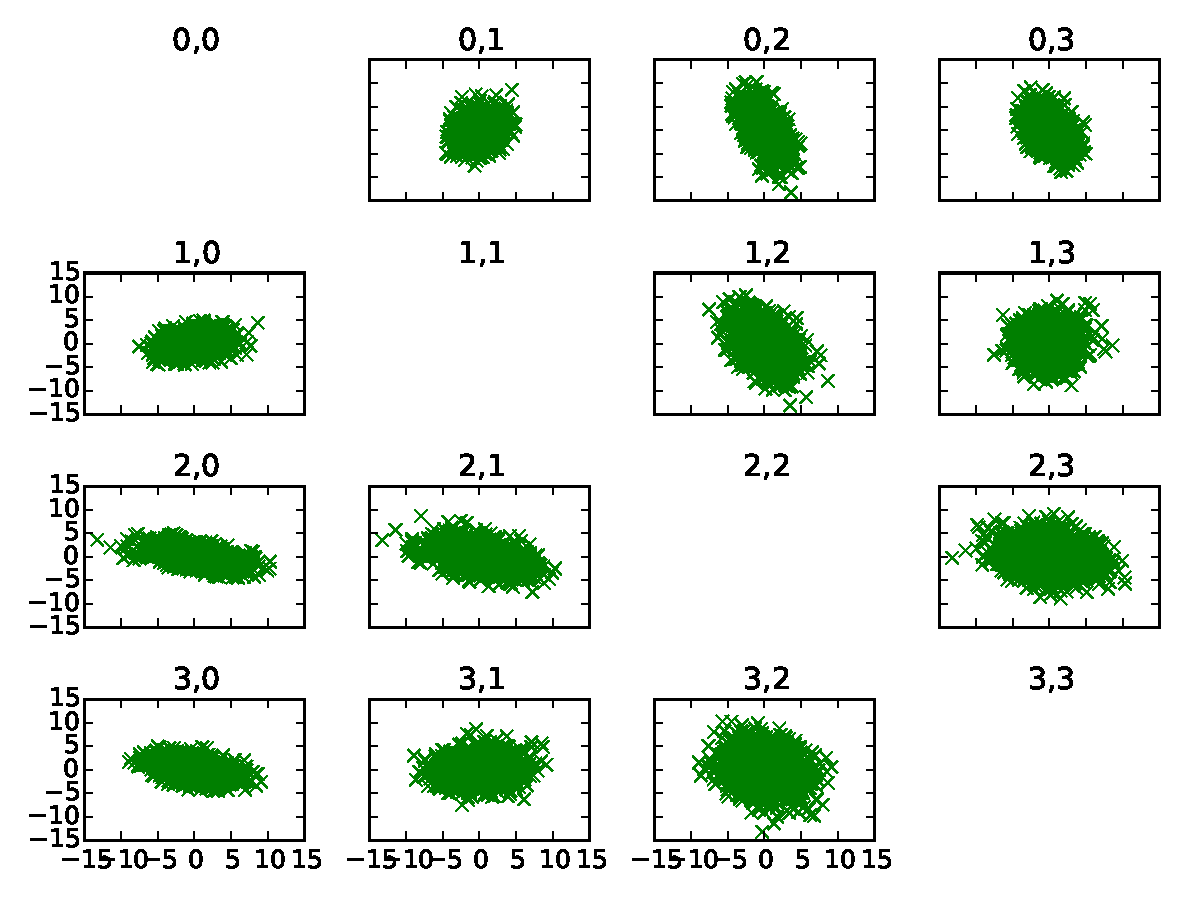
\includegraphics[width=\textwidth]{scatter.pdf}
\end{center}
\newpage
\section*{22 Exercise: Estimating mean($\vec{x}$) and covariance matrix (S)}
\begin{itemize}
\item
Below you can find the Maximum Likelihood estimator of the covariance matrix from a sample of n observations.
$$\widehat{\boldsymbol\Sigma} = {1 \over n}\sum_{i=1}^n ({\mathbf x}_i-\overline{\mathbf x})({\mathbf x}_i-\overline{\mathbf x})^T$$
It was easy to see that when the program was run with more draws the relative accuracy of the estimated mean and covariance matrix increased by differing less of the original $\mu$ and $\Sigma$.
\item
\inputminted{python}{E22.py}
\end{itemize}

\end{document}
